\documentclass[../Text/00main.tex]{subfiles}
\graphicspath{{../}}

\begin{document}

\section{Forward modelling}

The numerical simulation of an earthquake is a case of \textit{forward modelling}: the seismic source initiates a wavefield that propagates through a given model, and is recorded by receivers positioned in that model domain. The recorded data $\textbf{d}$ is generated by a forward modelling operator $\textbf{G}$ acting on model parameters $\textbf{m}$:

\begin{equation}
    \textbf{d} = \textbf{G}\textbf{m}.
\end{equation}

The $\textbf{G}$ operator in the case of numerical modelling of earthquakes represents the physics behind the wave propagation, here the elasto-dynamic propagation of seismic waves through a model domain with a given velocity model. The model parameters that we are interested are the source parameters. It is the question how detailed the model parameters in $\textbf{m}$, as well as the physics described in $\mathbf{G}$ need to be, in order to reproduce data $\mathbf{d}$ that is sufficiently in line with reality regarding the purpose that it is modelled for. The opposite of forward modelling is \textit{inverse modelling}

\begin{equation}
    \textbf{m} = \textbf{G}^{-1} \textbf{d}.
\end{equation}

Here, the data $\mathbf{d}$ is used in combination with the inverse modelling operator $\mathbf{G^{-1}}$ to obtain the model or source parameters $\mathbf{m}$. In this study, we use the model parameters of the source that were obtained by inverse modelling as input for our forward model. 


\section{The seismic moment tensor}\label{sec:CMTexplanation}

The seismic moment $M_0$ is a measure of the strength of an earthquake, usually given in dyne-cm (1 dyne = $10^{-5}$ N) or N m. It is a parameter introduced by \citet{aki1966generation} that is proportional to the amount of slip along a fault and the fault area:
\begin{equation}
    M_0 = \mu AD = \mu \times \text{fault area} \times \text{fault slip}.
    \label{eq:momentfault}
\end{equation}
with $\mu$ the shear modulus of the crust in the fault area. The seismic moment spans a large range of magnitude orders, typically from $10^5$ in laboratorial microfractures to $10^{30}$ in large earthquakes \citep{aki_quantitative_2002}. For these larger earthquakes, based on the seismic moment often a moment magnitude $M_w$ is published. This is a scale of the earthquake magnitude, given in N m by \citet{hanks1979moment} as
\begin{equation}
    M_w = \frac{2}{3}(log_{10} M_0 - 9.1).
\end{equation} 



The seismic moment tensor $M_{ij}$ is a mathematical representation of the moment generated by a seismic source, and comprises an integral over the moment tensor density $m_{ij}$ for a given source volume $\text{V}$ or a surface density $m'_{ij}$ internal surface $\Sigma$

\begin{equation}
    M_{ij} = \int_{V} m_{ij} dV = \int_{\Sigma} m'_{ij}.
\end{equation}

\citep{backus_moment_1976} have shown that the seismic moment tensor represents the non-elastic deformations in the source region, given by the stress $\sigma_{ij}$ in exess of purely elastic stress $\tau_{ij}$, also named the \textit{stress glut}. 
\begin{equation}
    m_{ij} = \tau_{ij} - \sigma_{ij}.
\end{equation}
For a given medium, displacements by impulsive forces acting at a point are represented by Green's functions. The spatial derivatives of this Green's function represent displacements caused by double couples or dipoles of these impulsive forces. The first-order moment tensor contains the first derivatives of the Green's functions, and higher-order moment tensors contain further derivatives of the Green's functions that are then also dependent on the moment tensor variations in space and time. This indicates that the moment tensor can encompass different types of sources: point sources as well as extended sources in space and time. We consider a first-order moment tensor $M_{ij}$, representing the source acting at a single point. The nine elements of this second-order tensor describe nine generalised force couples \citep{richards1980quantitative}, see Figure \ref{fig:mtcomponents}, with linear vector dipoles on the diagonals and force couples with an arm at the off-diagonals. These couples can be represented in both a Cartesian (x,y,z) frame as by a spherical coordinate system (r, $\phi$, $\theta$) and are given by:

\begin{equation}
M_{i j}=\left[\begin{array}{lll}M_{11} & M_{12} & M_{13} \\ M_{21} & M_{22} & M_{23} \\ M_{31} & M_{32} & M_{33}\end{array}\right] 
\quad 
\xrightarrow[\text{spherical}] 
\qquad 
\left[\begin{array}{lll}M_{r r} & M_{r \theta} & M_{r \varphi} \\ M_{\theta r} & M_{\theta \theta} & M_{\theta \varphi} \\ M_{\varphi r} & M_{\varphi \theta} & M_{\varphi \varphi}\end{array}\right],
\label{eq:matrixmt}
\end{equation}


with on the right the components in spherical coordinates ($r, \varphi, \theta$) representing (up, south, east), when following the Global CMT and Harvard conventions. The diagonal contains the isotropic parts and the off-diagonals contain the deviatoric parts of the tensor, see Figure \ref{fig:cmtseparatecombine}. The condition of zero net moment is applied to the moment tensor so that $m_{ij}=m_{ji}$, rendering it a symmetric tensor. The symmetry of the tensor makes for six individual moment tensor components ($m_{rr}, m_{tt}, m_{pp}, m_{rt}, m_{rp}, m_{tp}$ in spherical coordinates) that are linearly related. See the visualisation in Figure \ref{fig:cmtseparatecombine}. 

\begin{figure}[htb!]
    \centering
    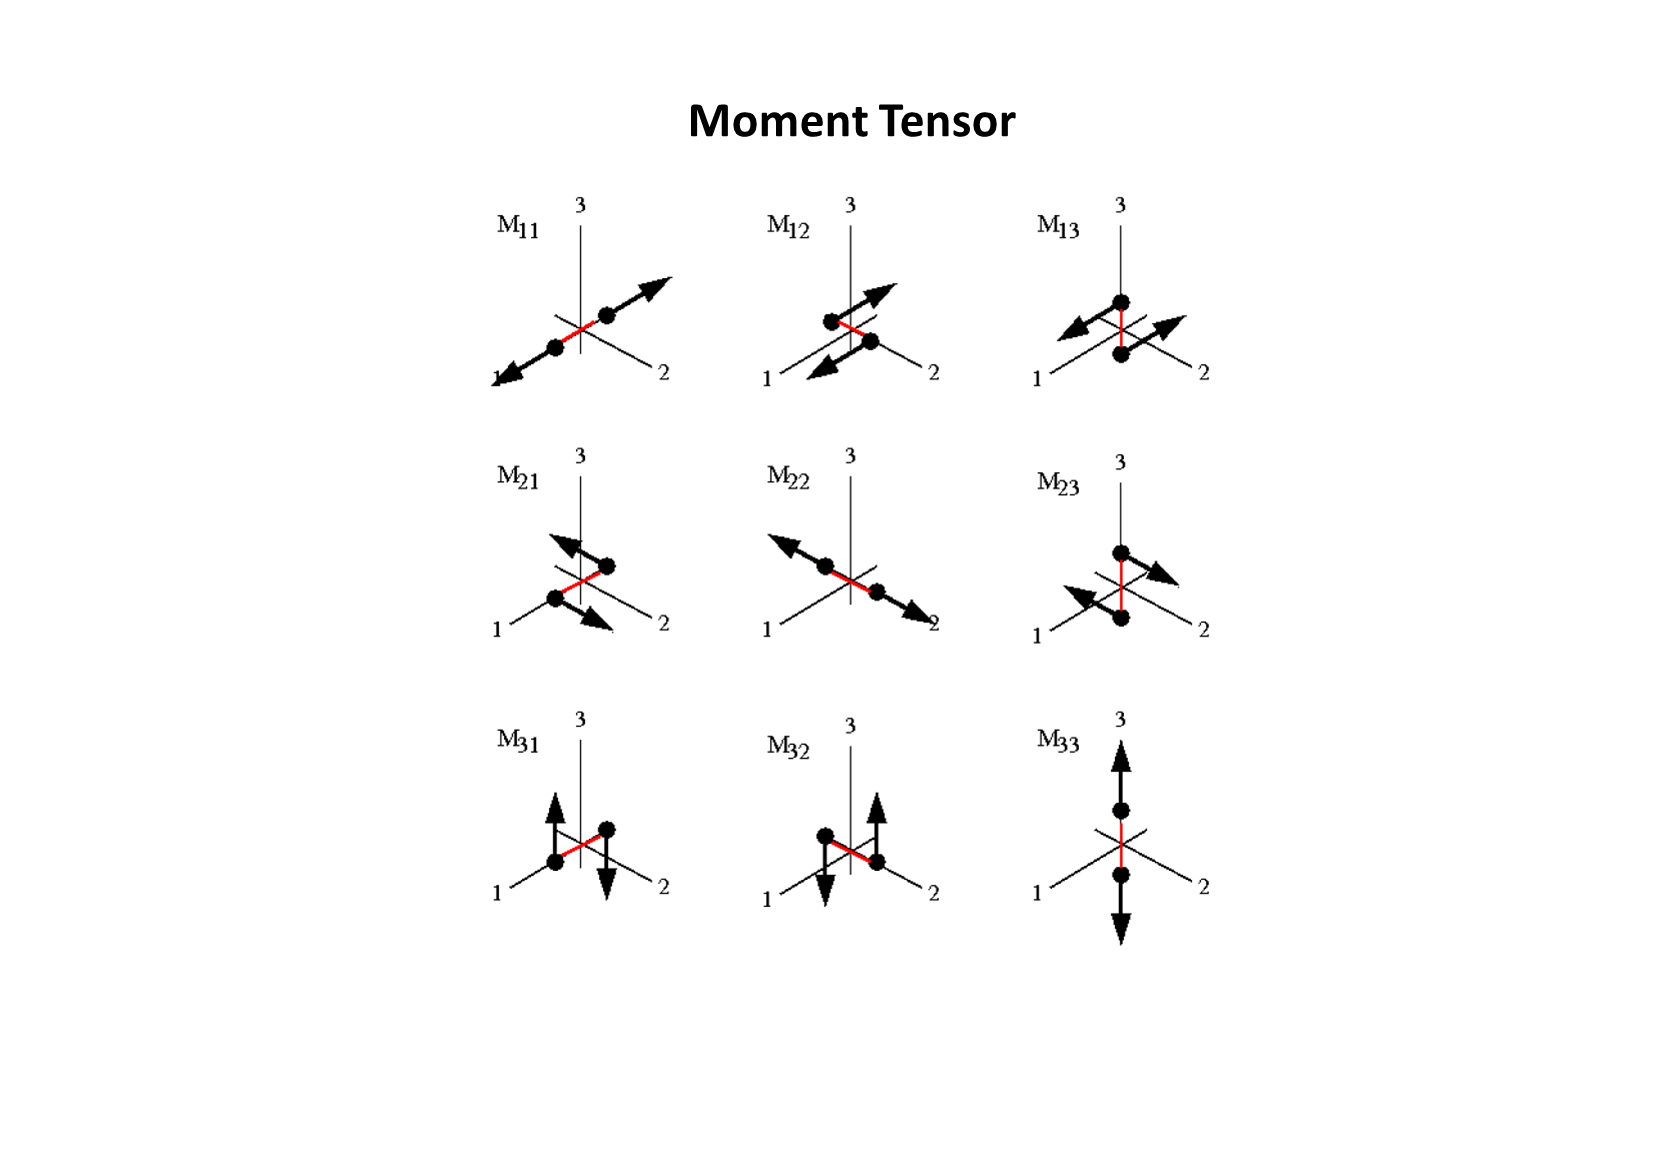
\includegraphics[width=.5\linewidth, trim = 6cm 3cm 5cm 3cm, clip]{images_methods/Stress-and-Moment-Tensors.png}
    \caption{The nine linear vector dipoles represented by the moment tensor. Mind that for the Harvard convention, such as in equation \ref{eq:matrixmt}, the subscripts ($r, \theta, \phi$) correspond to (up, south, east) in this image (3, 1, 2). }
    \label{fig:mtcomponents}
\end{figure}

\begin{figure}[htb!]
    \centering
    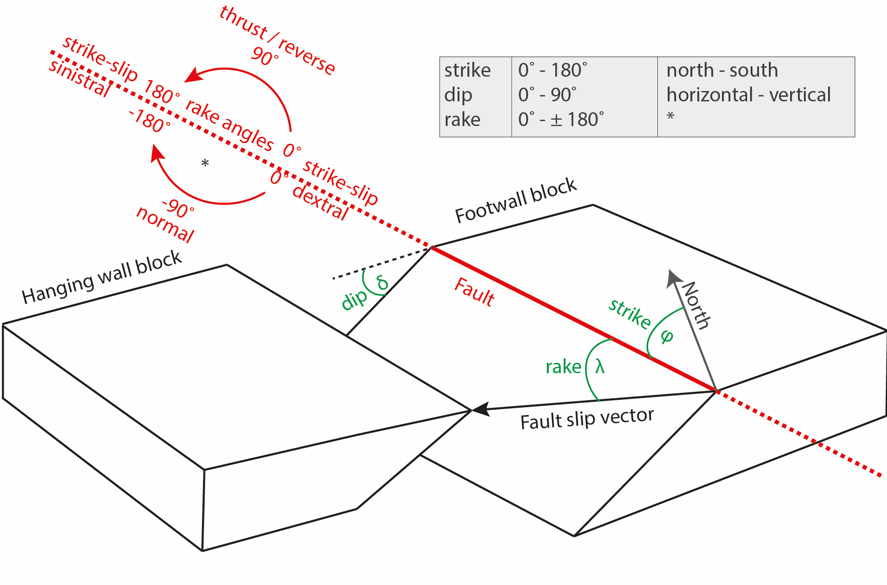
\includegraphics[width=0.75\textwidth]{images_methods/sdr_explainfig.png}
    \caption{Visual explanation of the strike, dip and rake angles in an abstracted view of a seismic fault rupture.}
    \label{fig:sdr_explainfig}
\end{figure}

The source type is now characterised by the six linearly related moment tensor components, and can represent explosions or implosions when it is purely isotropic, a pure shear dislocation source when it is purely deviatoric, or a mix between a deviatoric and isotropic source. For the source of a tectonic earthquake, a source that is (close to) a \textit{shear fracture} is often assumed. This means that the net volume change is zero or close to zero, as the high compressive stress allowing for little to no volume change. An earthquake along a fault can be described in terms of its angle with respect to the north (strike, $\varphi$), its angle with respect to the horizontal surface (dip, $\delta$), and the direction of slip along the fault plane (rake, $\lambda$). This is visualised in Figure \ref{fig:sdr_explainfig}. The six moment tensor components can be computed by the strike, dip and rake angles of an event, scaled by the scalar seismic moment $M_0$ as such \citep{udias2014source}:

\begin{equation}
\begin{array}{l}
m_{11}=- M_0 \sin \delta \cos \lambda \sin 2 \phi- M_0 \sin 2 \delta \sin ^{2} \phi \sin \lambda, \\
m_{22}= M_0 \sin \delta \cos \lambda \sin 2 \phi- M_0 \sin 2 \delta \cos ^{2} \phi \sin \lambda, \\
m_{33}= M_0 \sin 2 \delta \sin \lambda \\
m_{12}= M_0 \sin \delta \cos \lambda \cos 2 \phi+ M_0 \frac{1}{2} \sin 2 \delta \sin 2 \phi \sin \lambda, \\
m_{13}=- M_0 \cos 2 \delta \sin \lambda \sin \phi- M_0 \cos \delta \cos \phi \cos \lambda, \\
m_{23}= M_0 \cos 2 \delta \sin \lambda \cos \phi- M_0 \cos \delta \sin \phi \cos \lambda.
\end{array}
\end{equation}

Note that for using the Harvard or GCMT convention, 1 = $\theta$, 2 = $\phi$ and 3 = r. 

\begin{figure}
    \centering
    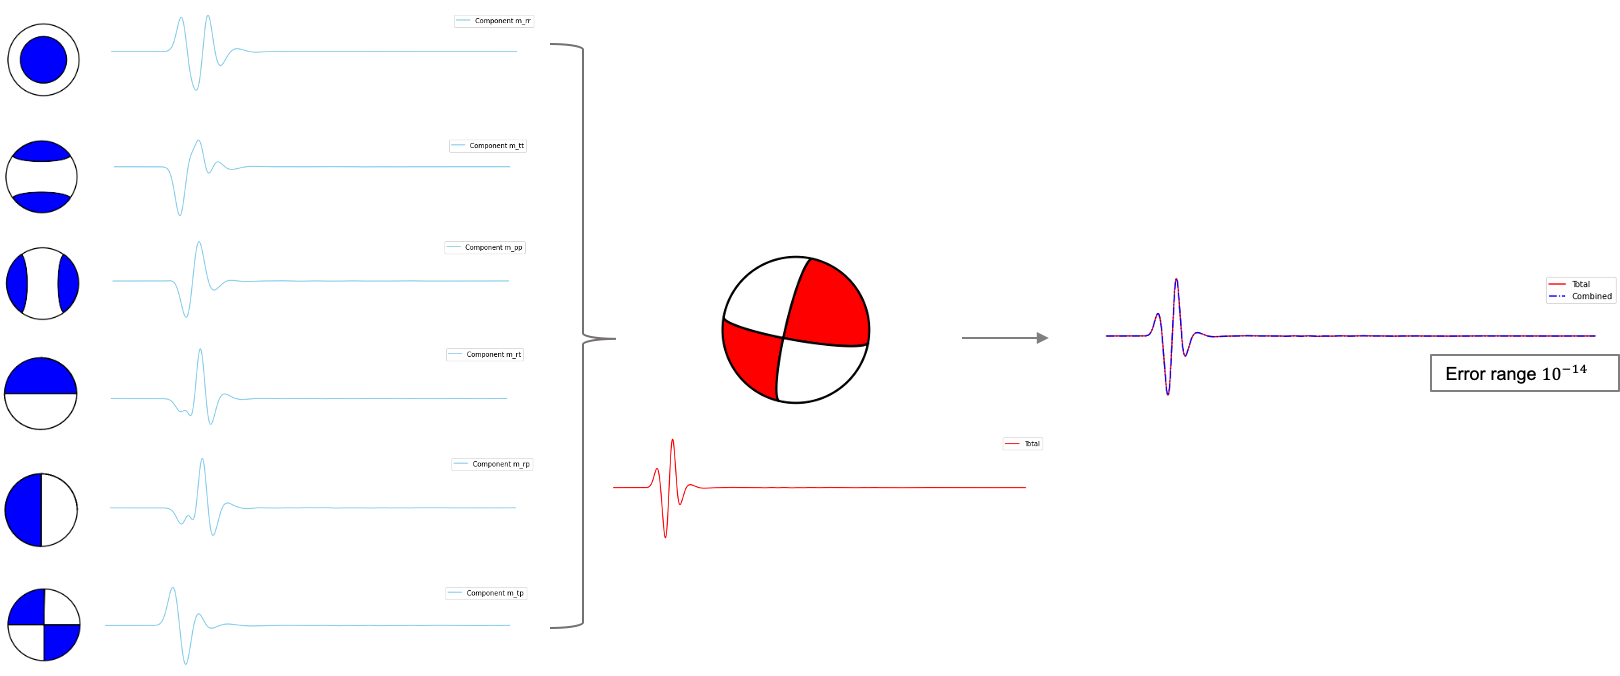
\includegraphics[width=.85\textwidth]{images_methods/cmtcombi_informationfigure.png}
    \caption{The six CMT components represented by their respective focal mechanisms. They can be summed to create the total moment tensor. When compared to the result of a simulation run with a total moment tensor solution, the error is below the floating-point range.}
    \label{fig:cmtseparatecombine}
\end{figure}

%%%%%%%%%%%%%%%%%%%%

\subsection{Radiation pattern}

The deformations excited by the source are radiated outwards from the source region in the form of seismic waves. These waves form a distinct pattern which is different for the direct source region and the far field. The relevant pattern here is the pattern recorded at the surface: the far-field pattern, and is given by a convolution of the spatial first derivative of the Green's function with the moment tensor at the source location $\mathbf{x_0}$ at source time $t_0$
\begin{equation}
u_{i}(\mathbf{x}, t)=G_{i j, k}\left(\mathbf{x}, t, \mathbf{x}_{0}, t_{0}\right) * M_{j k}\left(\mathbf{x}_{0}, t\right), 
\end{equation}
see \citep{aki_quantitative_2002}. Assuming a double-couple source with a strike, dip and rake such that we have a dextral strike-slip movement, the radiation pattern in the far field for a homogenous isotropic medium is depicted in Figure \hl{ref figure} and its shape is governed by the different wave-types. Longitudinal P-waves and Rayleigh surface wave radiate at an angle with respect to the fault surface, whereas the transverse waves such as S-waves and Love waves travel in the fault and fault-normal directions. The pattern changes when the strike, dip or rake of the source is altered, as well as the depth or at different frequency contents of the signal measured at the surface, see appendix \hl{Appendix patterns}. An analytical study of the surface wave patterns can be done using a homogeneous halfspace, but this becomes increasingly complex for heterogeneous media. A web-application has been developed by  \citep{rosler2020using} to directly see the influence of changing these parameters using a spherically symmetric earth model. One of the questions in this research is how the particular medium in question, the radially and laterally inhomogeneous subsurface of Istanbul, as well as the addition of topography at the surface and a fluid layer will affect this pattern. 

%%%%%%%%%%%%%%%%%%%%%%%

\subsection{Centroid moment tensor}

The Centroid Moment Tensor (CMT) approximation is a commonly used moment tensor for representing the seismic source of an earthquake as a point-source. The CMT lies at the \textit{centroid} of the fault rupture and is reccommended as the better source location of a finite rupture by \citep{dziewonski_determination_1981}. When using first-arrival P- or S-waves, the location of the seismic source when inverted for will be close to the initiation point of the rupture. The centroid could be described as the "centre of mass" of an event. For small events, this location will be close to the initiation location of the rupture. If using later-arriving phases in the surface wave, this location is shifted along the fault plane. The GCMT catalogue (GCMT, \citet{ekstrom2012global}, \citet{dziewonski_determination_1981}) inverts for the CMTs after a large seismic event and publishes the moment tensor solution online. The amount of coverage of an event by seismic stations grossly influences the quality of the source inversion. Not all events with a damage potential are captured by these catalogues, prompting the first workflow step of ChEESE as near-realtime source inversion. 

Realistically, a moderate (> $M_w$ 5.0) to large (> $M_w$ 6.0) event has a large rupture area, see Equation \ref{eq:momentfault}. The location of the seismic source is obtained by solving an inverse problem for a model vector $\mathbf{m}$($m_{11}$, $m_{22}$, $m_{33}$, $m_{12}$, $m_{13}$, $m_{23}$, centroid time, centroid latitude, centroid depth, centroid depth) containing the six moment tensor components, the lateral location, and the source depth. Inversion is done using long-period teleseismic data, in which the distance is much larger than the wavelengths considered. The wavetypes used for this are long-period body waves, which are the first arrivals, and surface waves with both a period of around 50 s. Additionallly mantle waves with a period around 135 s are used. With the inversion of the source using these wavetypes, the focal mechanism with the best fit or minimum misfit is chosen as the final focal mechanism. Uncertainty on the model parameters reported by the CMT catalogue is in the order of tens of kilometers for lateral location, in the order of kilometers for depth and in the order of fractions of a second for timing. These errors, including those on the six moment tensor components, are assumed to come forward from data modelling errors and do not take into account modelling errors caused by the relatively course subsurface PREM model often used in these inversions. \citep{valentine_assessing_2012} show that error estimates can increase substantially if modelling errors are also taken into account, and reccommend performing ones own inversion for purposes such as forward modelling where the source composition is important. In the pilot demonstrator for ChEESE, the first post-event step of an urgent seismic simulation is determining the CMT solution for the event source. The next step of the urgent seismic simulation protocol would be a more realistic source model with a finite rupture such as \citet{graves_kinematic_2016}. In these finite kinematic rupture simulations, the rupture of a large fault surface or series of fault surfaces itself is modelled with a fault of a certain roughness, length, depth, and a function governing slip propagation. However, the amount of parameters to be chosen, i.e. a much longer $\mathbf{m}$, and the high computational cost of this more realistic rupture model make this type of source modelling prohibitive to use when even the CMT solution is uncertain. The rapid post-event source estimates must therefore first provide a CMT solution.


\section{The spectral element method}

The spectral element method (SEM) is used as the numerical method to model the propagation of the seismic wavefield for our reference earthquake scenarios. SEM is a class of Finite Element Methods, benefiting from the implicit free surface property and it proves to be very well suited for discretisations of domains with complex topography \citep{fichtner_deep_2013}. Spatial discretisation of hexahedral elements and a Finite-Difference time-stepping method approximate the solution of the elastodynamic wave-equation at each point. The elastodynamic wave equation in 1D is given by

\begin{equation}
\rho \partial_{t}^{2} u + \partial_{x}\left(\mu \partial_{x} u\right) = f,
\label{eq:elastodynamic1D}
\end{equation}

with displacement $u(x,t)$, external force $f(x,t)$, density $\rho$, and shear modulus $\mu$. The discretised wave-equation is represented by the following global equation

\begin{equation}
    \mathbf{M}\partial^2_t\mathbf{u}(t) +
    \mathbf{Ku}(t) =
    \mathbf{f}(t),
    \label{eq:mutkutglobal}
\end{equation}

with $\mathbf{u}$ the unknown wavefield solved at each point, $\mathbf{K}$ the stiffness matrix, $\mathbf{M}$ the mass matrix (note that this is a different M than the seismic moment earlier) and $\mathbf{f}$ the volumetric force vector. It makes use of fourth-order Lagrange polynomials as interpolation functions, with Gauss-Lobatto-Legendre (GLL) collocation points. GLL points are the roots  of the first derivative of the Legendre polynomials and allow for an optimal spatial point distribution \citep{igel_spectral-element_2016}. Usage of these GLL points as quadrature points makes the mass matrix $\mathbf{M}$ diagonal and thus trivially invertible. Other type of meshes than hexahedral meshes can be used, but then this favourable diagonal property is lost. The time-stepping scheme allows for relatively straightforward paralellisation of simulations. The wavefield solution for the next time step $t + dt$ is computed as

\begin{equation}
\mathbf{u}_{g}(t+d t)= dt^{2}\left[\mathbf{M}_{g}^{-1}\left(\mathbf{f}_{g}(t)
-\mathbf{K}_{g} \mathbf{u}_{g}(t)\right)\right] 
+ 2 \mathbf{u}_{g}(t)-\mathbf{u}_{g}(t-d t) ,
\end{equation} 

where the subscript $g$ denotes that the solution is global. This time discretisation renders the method particularly suitable for large-scale wave propagation simulations that make use of HPC resources. The method was adapted for 3D wave propagation by \citet{komatitsch1999introduction} and is now one of the more widely used methods for deterministic seismic simulations. \citet{igel_spectral-element_2016} offers a more extensive explanation of the spectral element method. 


%%%%%%%%%%%%%%%%%%%%%%%%%%%%%%%%%%%%%%%%%%%%%%%%%%%%%%%%%
%%%%%%%%%%%%%%%%%%%%%%%%%%%%%%%%%%%%%%%%%%%%%%%%%%%%%%%%%

\section{Towards a realistic model domain: topography and ocean}

\subsection{Topography effects}

Topography has been proven to influence duration, spectral content, amplification and de-amplification of seismic waves, e.g. (\citet{veeraraghavan_simulation_2020}, \citet{pienkowska2020high}, \citet{stolte2017experimental}, \citet{imperatori2015role}). This may have significant effects on the intensity measures that are studied in the context of this thesis. \citet{veeraraghavan_simulation_2020} is an important study in relation to this thesis. Findings of this study are that the presence of topographical features cause backscattering of seismic waves towards the source. This backscattering decays quickly in a domain with homogeneous shallow subsurface, but addition of a detailed soil-layering causes more significant effects.  shows that amplification takes place at the ridges of topographical features, and de-amplification at the foot of steep topographical features, and that duration of the signal is elongated by the presence of topography. They also show that topographical features in the lateral extent have the most effect in close proximity to the source (< 2 km), whereas this range is larger for the vertical extent. Another important finding here is that intensities at large distance are more affected by the presence of topography than by the dip of the fault. \citep{imperatori2015role} shows that inclusion of topography can affect the patterns of PGV and lead to back-scattering towards the source and stresses the need for both a shallow soil layering model, as well as the inclusion of topography if this is a distinct feature in the domain at question. Primarily the sub-surface exhibits steep topography in the Marmara region considered here, as discussed in section \ref{CH1sec:Tectonics}. The spectral element method is well suited for domains with complex surface topography. The hexahedral elements at the surface can be deformed to the topography. 

\subsection{Oceanic coupling}

When modelling at periods < 10 seconds, crustal features, effects of a deep water layer in the domain as well as an undulating bathymetry, start to become increasingly important for realistic forward modelling. P-waves travelling up to the water surface and reflecting back into the crust, as well as frequencies travelling in the low-velocity SOFAR channel, that acts as a waveguide for low-period waves, can have a frequency content of a few seconds \citep{fernando2020oceanic}. The oceanic layer is however not straightforward to model. For example, it could be accounted for as an \textit{oceanic load} \citep{komatitsch2002spectral}. This entails accounting for the weight of the ocean by "loading" each surface node, and setting the shear modulus to zero at each point of the surface. This mitigates actually having to implement the ocean in the mesh. The formulation however only proves valid if the water column height is only a fraction of the dominant wavelength of the simulation \citep{fernando2020oceanic}. If the water column becomes sufficiently deep, or the dominant period increases above 20 s, simulations utilising a coupled solid-fluid simulation provide more accurate results. In the solid-fluid coupled simulation, the boundary condition at the surface changes from a Neumann free surface boundary condition, which was implicit in the spectral element formulation, to having to implement a Dirichlet pressure-free boundary condition at each point of the oceanic surface \citep{zhou_location_2016}. The bottom of the ocean, or the  top of the solid domain, is now not traction free, whereas the shear component here can be assumed zero.



The change is most dominant in the surface waves, which are highly relevant in the context of this study.  \citet{fernando2020oceanic} also shows that inclusion of realistic bathymetry contributes to better approximate the wavefield. This motivates to include these more realistic features into the domain of this study, as the dominant frequency is set at 1 Hz and a considerate portion of the domain surface is covered by the Marmara sea. This does however elevate computational costs. In addition to the deformed mesh due to undulating bathymetry, a finer discretisation in space and time have to account for the lower velocities in the water layer with smaller minimum wavelength.. 





\section{Ground motion parameters}

It is key to express the abundance of information that can be obtained from a seismogram as meaningful parameters. Ground motion parameters (GMP) or intensity measures (IM), are measures of the ground motions derived from these seismic records, or from civil surveys such as the USGS "Did You Feel It" index (DYFI, \cite{atkinson2007did}). The commonly analysed ground motion parameters derived from records can be sub-divided into three main categories: duration-based, peak-based and spectral parameters. In this section we explain the definition of the parameters used to compare to recorded data and map out the earthquake response in this study. 

\subsection{Peak Ground Acceleration (PGA)}

The Peak Ground Acceleration (PGA) corresponds to the highest amplitude of the acceleration time series of the earthquake signal at a given station. It is a much-used parameter in seismic hazard assessment and a map of the PGA is often published after a significant event:

\begin{equation}
    PGA = max(\mid a(t) \mid),
\end{equation}

with $a(t)$ the acceleration time series. The PGA is an indicator of the severity of the ground accelerations during an event, and is used for structural engineering purposes. However, the duration or spectrum of the event is not captured by this parameter. Thus, a high PGA does not always represent the same amount of damage. High-frequency content of the earthquake signal can cause high PGA values of a short duration. Very high PGA values in the range of 0.5-1.2 $g$ have been shown to cause only minor damage \hl{cite} due to their cause by short-duration higher-frequency content of the earthquake signal. The PGA is therefore mostly used for relatively short-period (> 2 Hz) waves and in earthquake engineering for shorter buildings \citep{kramer:1996}. It directly represents the force, in the two horizontal directions and the vertical direction, that a building is subjected to during an event. 

\subsection{Peak Ground Velocity (PGV)}

The Peak Ground Velocity (PGV) represents the highest amplitude of the velocity time series of the earthquake signal at a given station:
\begin{equation}
    PGV = max(\mid v(t) \mid),
\end{equation}

with $v(t)$ the velocity time series. The PGV is also used as damage indicator, and is less sensitive to higher-frequency content than the PGA. This is because signals with a low acceleration/velocity ratio generally have longer duration and energy at the lower end of the frequency spectrum (\citet{tso1992engineering}, \citet{kramer:1996}). The PGV is used for earthquake building engineering for the modelling of taller buildings or other longer-period structures in the intermediate frequency ranges (1-2 Hz), such as bridges hl{(how many stories?)}. It is one of the primary measures in more severe earthquakes \hl(reference?). PGD, which is only considered for waveform fit in this study, is a suitable measure for low-frequency ground motions.

\subsection{Spectral Response}

The spectral response is a popular parameter for earthquake engineering purposes. It represents the peak spectral acceleration $S_a$ for each frequency-band of the signal. The spectrum represents a series of single-degree-of-freedom (SDOF) oscillators that oscillate at their respective natural frequencies $\omega_0$ ($\omega_0 = 2\pi/T_0$), damped by a damping factor $\xi$. Spectral acceleration is calculatedby calculating the maximum absolute acceleration of the time series of a SDOF oscillator for each natural frequency. Somewhat easier to calculate is the pseudo-spectral acceleration that we will use in this thesis. For engineering purposes, with low damping ratios, the spectral and pseudo-spectral accelerations are assumed to be equivalent \citep{newmark1974fundamentals}. The pseudo-spectral acceleration $Ssa$ makes use of the spectral displacement $S_d$ which is the absolute maximum displacement at a given period T. Undamped spectral acceleration is given by

\begin{equation}
    Ssa(T, \xi) = \omega^2 S_d(T, \xi).
\end{equation}

The pseudo-spectral acceleration is often used for modelling the force a building is subjected to during an earthquake. The damping factor represents the energy dissipation that occurs as the structure bends, causing the oscillations to decrease with time. It is common in structural engineering to use a 5\% minimum damping factor for seismic design, which is a value adopted in seismic hazard analysis. Pseudo-spectral acceleration spectra (Ssa) are plotted against natural periods $T_d$. 

\subsection{Arias Intensity}

The Arias intensity, introduced by \citet{arias1970measure}, is a measure of the intensity of a signal and its impact for a uniform population of structures. The intensity is an of the integral over the acceleration time series $a$ squared for the duration of the signal $T_d$, multiplied with  $\frac{\pi}{2}$:

\begin{equation}
    I_A = \frac{\pi}{2g} \int_0^{T_d} a(t)^2 dt
\end{equation}

with $g$ the acceleration of gravity. The measure captures the amplitude, duration and frequency content of the signal and is a common proxy used in earthquake engineering \citep{howard2008probabilistic}. It captures well the short-period structural response \citep{travasarou2003empirical}. 

\subsection{Energy integral}

The Energy integral is similar to the Arias intensity, and gives the total energy over the duration of the velocity time series. 

\begin{equation}
    I_E = \int_0^{T_d} v(t)^2 dt
\end{equation}

Both the Arias intensity and the energy integral are used in the GoF analysis of this project. 

\end{document}